\documentclass[handout,t]{beamer}
\usetheme[cabin, darktitle]{UniversityOfManchester}

%% Document properties
\title{An efficient SpiNNaker implementation of the Neural~Engineering~Framework}
\author{Andrew Mundy, James Knight,\\Terry Stewart and Steve Furber}

\usepackage{amssymb}
\usepackage{booktabs}
\usepackage[binary-units]{siunitx}
\usepackage[backend=bibtex, doi=false, url=false,
            autocite=footnote, maxbibnames=3, style=authoryear]{biblatex}
\bibliography{paper}

\renewcommand{\vec}{\mathbf}
\newcommand{\semanticpointer}{\textbf}
\newcommand{\msemanticpointer}[1]{\mbox{\semanticpointer{#1}}}

\begin{document}
  \maketitle

  %% Constraints on SpiNNaker programs
  %% - Memory usage
  %%  - In its own right
  %%  - Time to load data
  %% - Processing time
  %%  - Dominated by synaptic weight lookup -- < 5000 synaptic events per timestep
  \begin{frame}{Simulating neural nets on SpiNNaker}
    \vfill
    \hspace*{-.15\textwidth}\includegraphics[page=2, width=1.3\textwidth]{algorithm_diagram}
    \vfill
    \pause
    Constraints on number of neurons per core:
    \begin{description}
      \item[Memory] Size of weight matrix
      \item[Compute] Number of synaptic events
    \end{description}
  \end{frame}

  \begin{frame}{Performance of the SpiNNaker architecture}
    Constraints:
    \begin{itemize}
      \item \SI{8}{\mebi\byte} limit on weight matrices.
      \item Max \num{5000} synaptic events per millisecond \parencite{Sharp2013}.
    \end{itemize}

    \pause
    Overcome by:
    \begin{itemize}[<+->]
      \item Allocating fewer neurons to a core
        \begin{itemize}
          \item \textbf{but} power and number of processors limited.
        \end{itemize}
      \item Using longer simulation time-steps
        \begin{itemize}
          \item \textbf{but} sometimes hard deadlines.
        \end{itemize}
    \end{itemize}
  \end{frame}

%  \begin{frame}{Bad characteristics}
%    Fine for the majority of the cases, not helped by:
%    \begin{itemize}
%      \item Dense weight matrices
%      \item High firing rates
%    \end{itemize}
%    \pause
%    Both characteristics of models built with the Neural~Engineering~Framework~(NEF)
%  \end{frame}

  %% Introduction to the NEF
  \begin{frame}{The Neural Engineering Framework (NEF)}
    \begin{itemize}
      \item Populations of neurons represent abstract values.
      \item Connections compute functions of representations.
      \item Extended by the Semantic Pointer Architecture (SPA).
        \begin{itemize}
          \item Used to build Spaun, ``the world's largest functional brain model''
        \end{itemize}
    \end{itemize}
  \end{frame}

  %% - Encoding
  %% - Decoding
  %% - Forming weight matrices
  %% TODO Motivate encoding, explain decoding
  \begin{frame}[plain]{Representing scalars}
    \vfill
    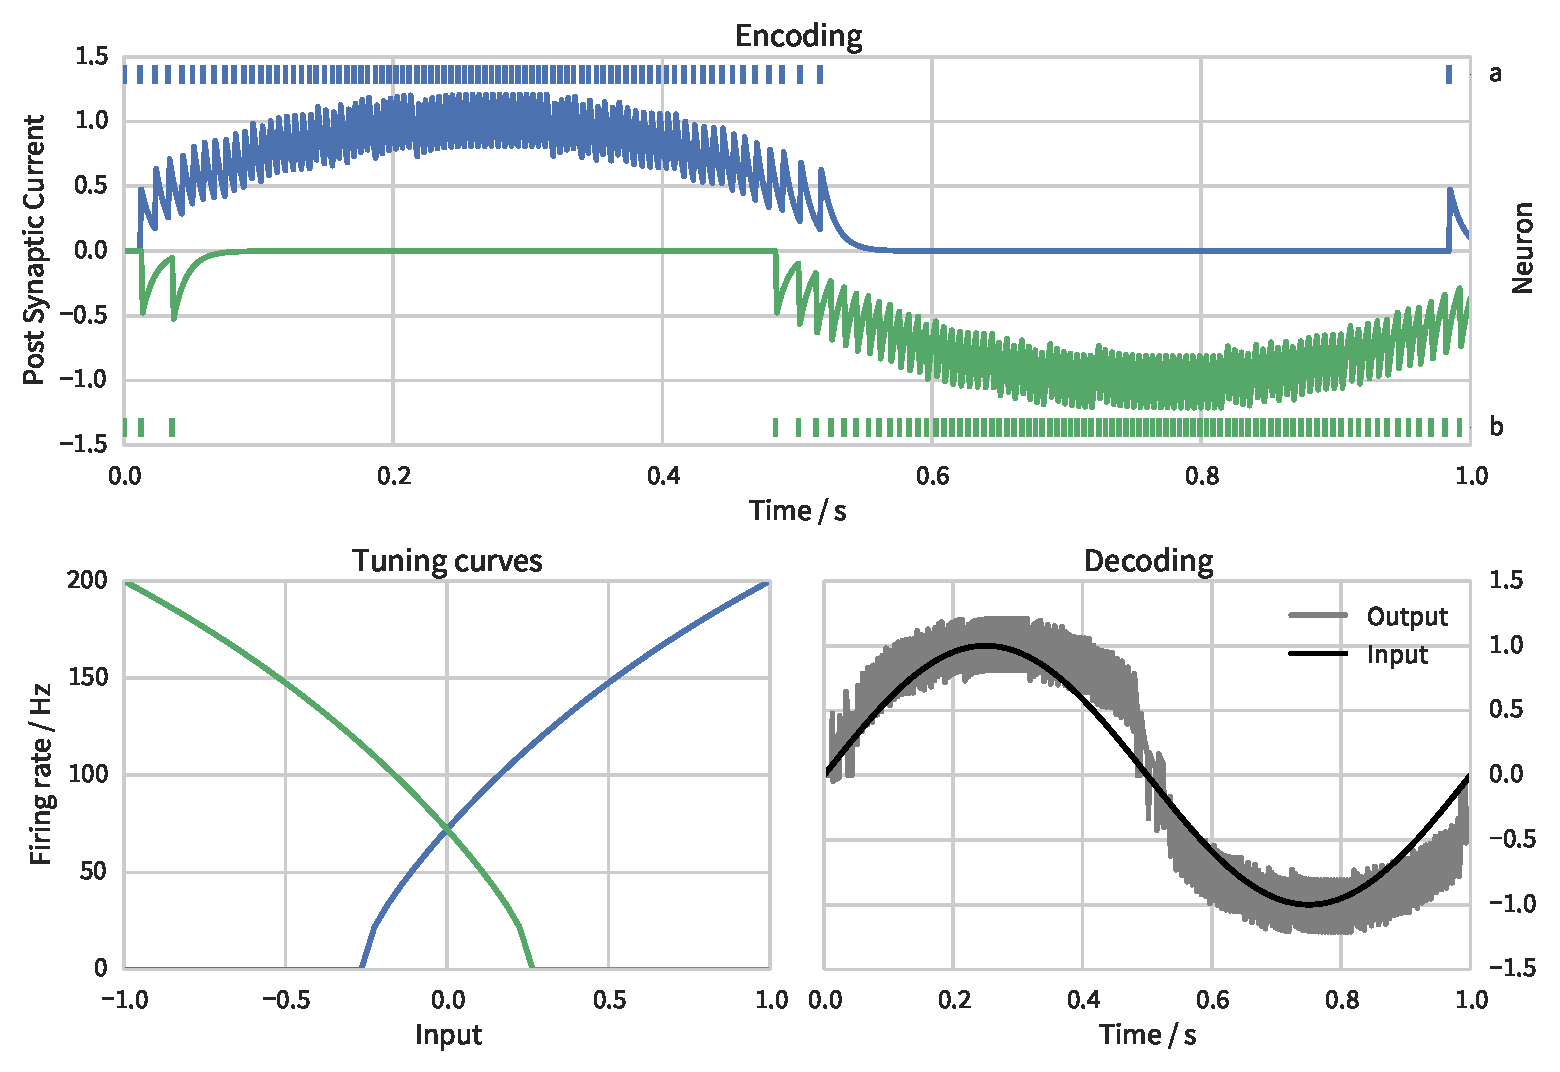
\includegraphics[width=\textwidth]{encoding_decoding}
    \vfill
  \end{frame}

  \begin{frame}[plain]{Representing vectors}
    \vfill
    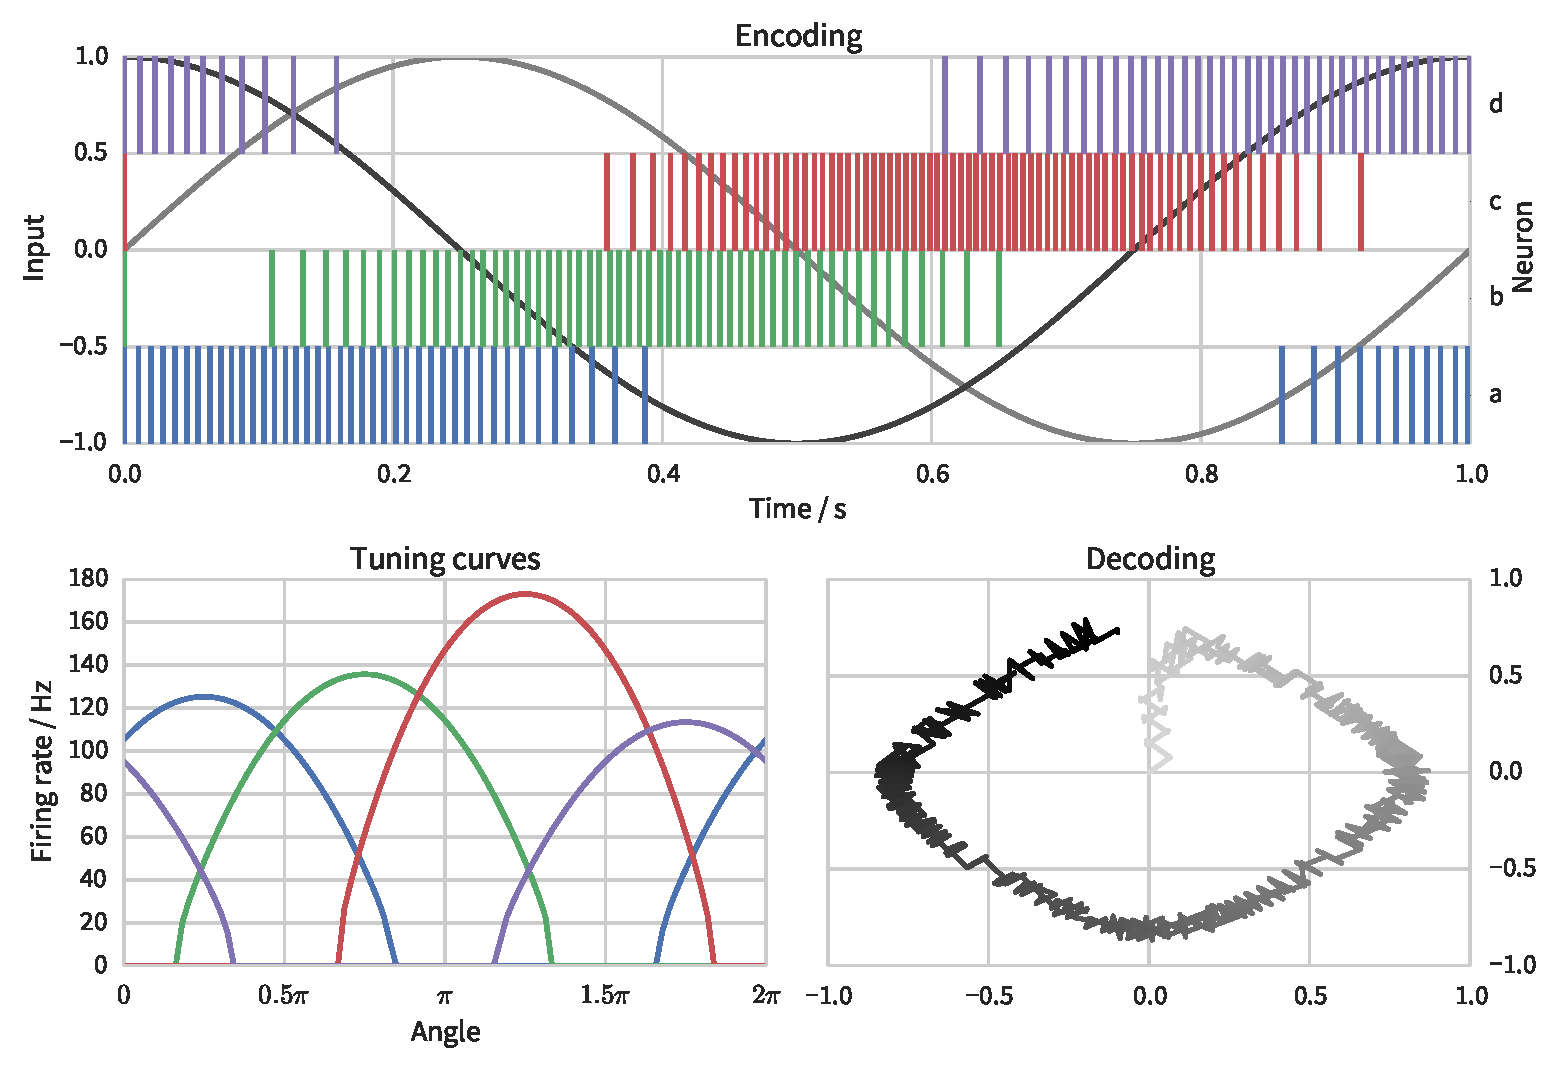
\includegraphics[width=\textwidth]{encoding_decoding2d}
    \vfill
  \end{frame}

  \begin{frame}{Combining encoding and decoding}
    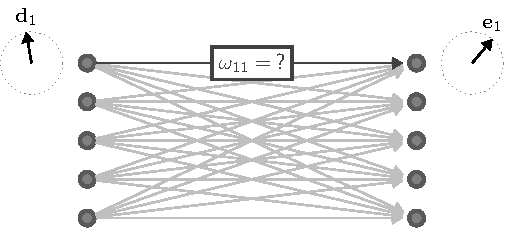
\includegraphics[width=\textwidth]{weight_matrices}

    \begin{itemize}
      \item Synaptic weights show the degree of similarity: $\omega_{ij} = \vec{d}_i \cdot \vec{e}_j$
    \end{itemize}
  \end{frame}

  \begin{frame}{The Semantic Pointer Architecture (SPA)}
    Represent concepts using high dimensional vectors, e.g.:
    \begin{align*}
      \msemanticpointer{X} &= \msemanticpointer{BLUE}\circledast\msemanticpointer{TRIANGLE} \\
                           &+ \msemanticpointer{RED}\circledast\msemanticpointer{SQUARE}\\
                           &+ \msemanticpointer{GREEN}\circledast\msemanticpointer{CIRCLE}
    \end{align*}

    Query with inverse: ``What shape is red?''
    \begin{align*}
      \msemanticpointer{X} \circledast \msemanticpointer{RED}^\prime &\approx \msemanticpointer{SQUARE}
    \end{align*}
    Result needs ``cleaning up''.
  \end{frame}

  \begin{frame}{Requirements of the NEF}
    General requirements:
    \begin{itemize}
      \item Weight matrices are dense
      \item High firing rates (typically upto \SI{400}{\hertz})
    \end{itemize}

    Heuristics for SPA:
    \begin{itemize}
      \item 70 neurons per dimension
      \item 500 dimensions for a human size vocabulary
    \end{itemize}
    \pause
    \textbf{Result: Poor use of the SpiNNaker architecture}
  \end{frame}

  %% How does the NEF meet these constraints?
  %% - Consider communication channel using Spaun-like parameters of 16-D and 70 neurons per dimension
  %%  - Memory use is insane (down to 53 neurons per core)
  %%  - Synaptic events very quickly pass the max allowed
  %% Result: using the standard approach with the NEF will lead to suboptimal use of the architecture.
  \begin{frame}{NEF on SpiNNaker -- Memory usage}
    Communication channel:
    \begin{itemize}
      \item Two populations representing 500 dimensions
      \item Each population has $70 \times 500 = \num{35000}$ neurons
      \item $\omega$ of order $\num{35000} \times \num{35000}$
      \begin{itemize}
        \item contains \num{1.225d9} elements
        \item at \SI{16}{\bit} per synapse = \SI{2.28}{\gibi\byte}
      \end{itemize}
      \item \textbf{Fewer than 119 neurons per core}
    \end{itemize}

    \vfill
    {\footnotesize Being kind and using dense matrices!}
  \end{frame}

  \begin{frame}{NEF on SpiNNaker -- Processor usage}
    Dominated by synaptic weight lookup --
    \begin{itemize}
      \item max 5000 synaptic events per millisecond
      \item NEF models have high firing rates -- typically up to \SI{400}{\hertz}
    \end{itemize}

    Communication channel:
    \begin{itemize}
      \item Two populations representing 4 dimensions
      \begin{itemize}
        \item 280 neurons per ensemble
      \end{itemize}
      \item $\approx 20$ incoming spikes per millisecond
      \begin{itemize}
        \item \num{5600} synaptic events per millisecond
      \end{itemize}
    \end{itemize}
  \end{frame}

  \begin{frame}{NEF on SpiNNaker}
    \begin{itemize}
      \item Dense weight matrices
      \item High firing rates
    \end{itemize}

    Likely will not scale to simulating Spaun: \textbf{what to do?}
  \end{frame}

  %% An alternative: value-based transmission
  %% - Note that weight matrices can be factored into encoders and decoders
  %% - Indicate how this can be used in simulation using the payloads of MC packets
  \begin{frame}{Value Transmission}
    \vfill
    \hspace*{-.15\textwidth}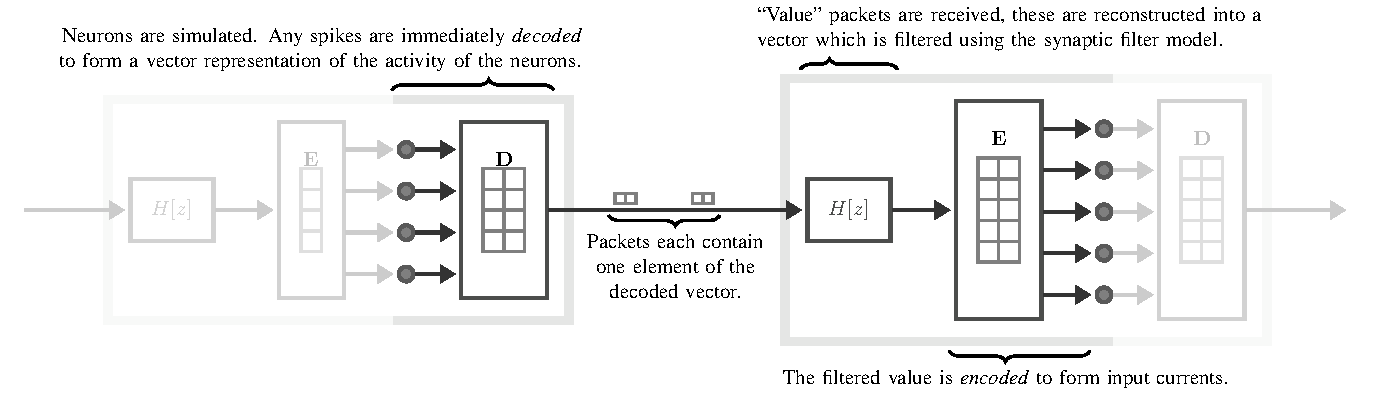
\includegraphics[page=1, width=1.3\textwidth]{algorithm_diagram}
    \vfill
    \pause
    \begin{itemize}
      \item Factored weight matrices $\ll$ full weight matrix
      \item Different compute requirements
    \end{itemize}
  \end{frame}

  %% Results
  %% - Memory usage
  \begin{frame}{Results -- Memory usage}
    Communication channel:
    \begin{itemize}
      \item Two populations representing 500 dimensions
      \item Each population has $70 \times 500 = \num{35000}$ neurons
      \item $\vec{D}$ and $\vec{E}$ of size $35000 \times 500$
      \begin{itemize}
        \item at \SI{32}{\bit} per value = \SI{133}{\mebi\byte}
      \end{itemize}
      \item \textbf{Around 2000 neurons per core} -- become compute bound before that!
    \end{itemize}
  \end{frame}

  \begin{frame}{Results -- Memory usage}
    Using basal ganglia model from Spaun:
    \begin{center}
      \begin{tabular}{r S S S S}
        \toprule
          Inputs & {16} & {32} & {64} & {128} \\
        \midrule
          Full weight matrix / \si{\mebi\byte} & 5.38 & 20.34 & 78.96 & 311.04\\
          Factored / \si{\mebi\byte} & 0.18 & 0.63 & 2.37 & 9.18\\
          Reduction / \si{\percent} & 96.71 & 96.89 & 96.99 & 97.05\\
        \bottomrule
      \end{tabular}
    \end{center}
  \end{frame}

  %% - Processor usage
  \begin{frame}{Results -- Processor usage}
    Using 70 neurons per dimension:
    \begin{itemize}
      \item Standard SpiNNaker scheme:\\
        $128N + 3N^2$ cycles
        \begin{itemize}
          \item Max of 236 neurons per core
        \end{itemize}
      \item Value-based scheme:\\
        $533 + 80N + 0.19N^2$ cycles
        \begin{itemize}
          \item Max of 834 neurons per core
        \end{itemize}
    \end{itemize}

    With 1-D representations: \textbf{2000 neurons per core}.
    \vfill
    {\small\color{black!60!white} Real-time using \SI{1}{\milli\second} time-steps, processor running at \SI{200}{\mega\hertz}.}
  \end{frame}

  \begin{frame}{Conclusion}
    \begin{itemize}
      \item Characteristics of the NEF lead to inefficient use of SpiNNaker
      \begin{itemize}
        \item Dense weight matrices
        \item High firing rates
      \end{itemize}
      \item Factored weight matrices
      \begin{itemize}
        \item Change nature of communication, \textbf{but}
        \item Reduce memory usage
        \item Increase number of neurons per core (up to 2000)
      \end{itemize}
    \end{itemize}
  \end{frame}

  \begin{darkframes}
    \begin{frame}
      \centering
      \vfill
      {\Huge Thank You}\\\vskip\baselineskip
      {\Large Any questions?}
      \vfill
    \end{frame}
  \end{darkframes}

  %% Thanks!
\end{document}
